\chapter{Evaluation Scheme} \label{chap:evaluation-scheme}

\section{Considered Platforms}
As the concept of using stream as a source of truth gains more attention and becomes more popular, many projects aiming at creating a processing platform evolving around streams started to take shape. 
Many companies first started their projects as in-house products and then later open-sourced them to enhance the development pace with the help of community. Kafka, which was first developed at LinkedIn, is the first prominent name in the field \cite{apachekafka}. It was later open sourced to the Apache Software Foundation. Yahoo! also created their own stream processing platform named Pulsar and it is now also an Apache project \cite{apachepulsar}. The company Alibaba also joins the trend by open sourcing their RocketMQ to Apache Foundation \cite{rocketmq}. In addition, there is the NATS streaming server, which is developed and maintained by the company Synadia on top of NATS messaging system to provide stream processing capability \cite{natsstreaming}. It is currently an incubating project of Cloud Native Computing Foundation. Pravega is also a quite new open-source project in the field \cite{pravega}. 

Since an adequate evaluation for all these platforms could not be contained within the scope of the thesis, only three platforms will be selected based on a set of criteria indicating the maturity, the size of the active community, the popularity of the platform and the quality of documentation.

Maturity is evaluated based on the project stage in an open source foundation if it belongs to one and the date of the first release. Because each project has different in-house phase before open-sourcing, the date of release on GitHub is chosen as the standardized criterion.

The size of active community is determined by the number of contributors of the project on GitHub and the number of related questions on Stackoverflow.

To assess the popularity, the number of GitHub stars and Google trend points of each project in the last 12 months are used.

The result of the preliminary evaluation is summarized in Table \ref{table:preliminary}. The data and number presented in the table were collected in 11/2020.

\begin{table}[h]
	\caption{Preliminary evaluation of 5 open-source ESP platforms.}
	\label{table:preliminary}
	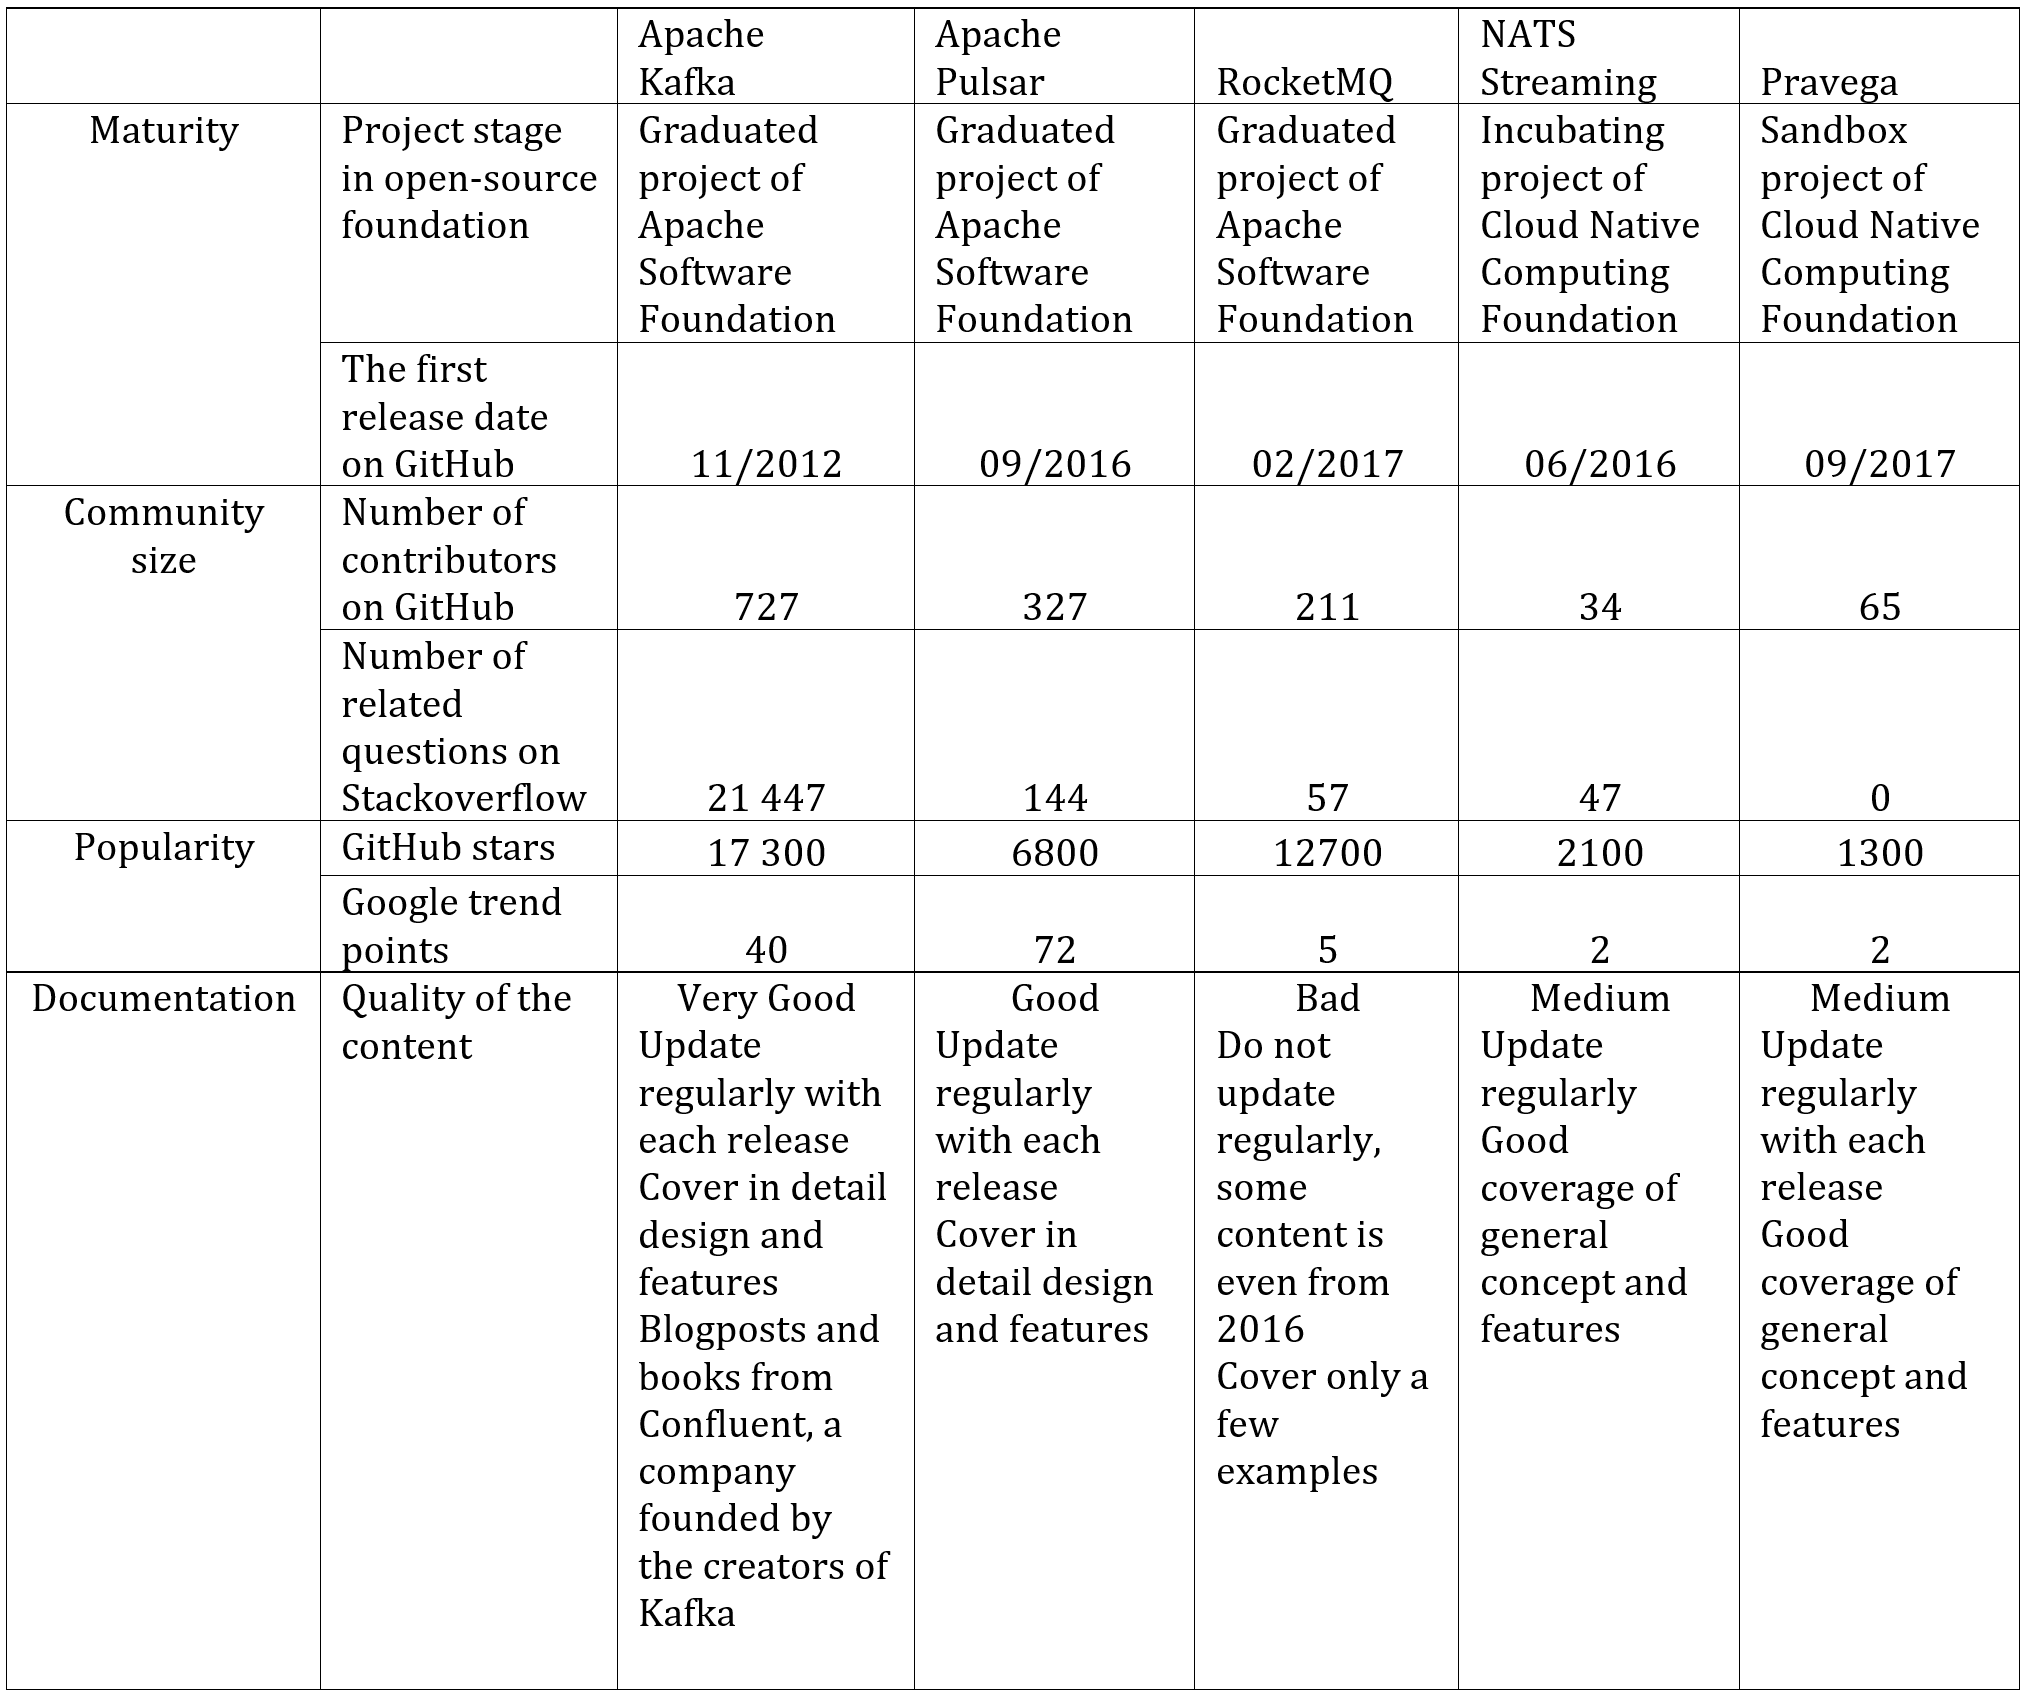
\includegraphics[width=\linewidth]{images/preliminary}
\end{table}

According to these criteria, Apache Kafka and Apache Pulsar are the leaders in all preliminary categories. Among the three remaining platforms, RocketMQ is the most popular in the community. However, the document page of RocketMQ is unfortunately very inadequate and outdated. This could become a great problem during the evaluation.  Therefore, RocketMQ will not be considered in the thesis. Regarding Pravega, despite the promising set of rich features, it is not mature enough since it is still in the sandbox stage at the Cloud Native Computing Foundation. Moreover, the community of Pravega is still too small. On the other hand, although NATS streaming has a moderate community, it has a reasonable maturity and quality of documentation. Moreover, it is built on top of NATS messaging system which is used in industry by many companies such as Siemens, Pivotal, GE and therefore can inherit its stability. The evaluation of NATS streaming can be greatly beneficial for organizations which already have NATS messaging in the infrastructure to integrate NATS streaming more easily.

As a result, the three platforms which will be inspected in depth are Apache Kafka, Apache Pulsar and NATS streaming.

\section{Evaluation Metrics}
The evaluation categories for distinct functionalities of an ESP platform are derived based on the necessary capabilities in section \ref{section:general-ESP-platform}. Since there are not many major scientific works on evaluating ESP platforms, concrete criteria which are directly related to ESP platforms cannot be found. Therefore, criteria in these categories are determined mainly by self-deducing from the literature research of related technology to each capability of an ESP platform or event-driven concept and from interviewing with experts at the company Novatec who work intensively with ESP platforms.

For general functionalities such as security and non-functional criteria, the comparison categories are adapted from ISO25010 software quality model to have a good coverage of main quality aspects \cite{iso25010}. However, non-applicable characteristics from the standard such as maintainability which refers to the inner structure and complexity of the system will not be included. As a result, 12 main comparison categories are determined. 

\textbf{1: License:}

1.1: Open-Source license: there are many open-source licenses available and each of them can impose some restriction on the use of the platforms. Users can have different intentions when using an open-source ESP platform such as for internal use or to build a commercial product on top of it. Therefore, this criterion is added to help users quickly decide which platform has the suitable license for their business model. It will not contribute to the points of the platforms in the evaluation. 

\textbf{2: Event storage}: this category is directly corresponding to the event store capability of the platforms. In this category are the criteria to evaluate this storage functionality.

2.1: Durable storage: with event-driven application, the event stream is the backbone that all application and services depend on. Therefore, events on an ESP platform must be stored in non-volatile storage. It must be guaranteed that once an event is confirmed to be persisted, it must survive system crash or power outage.

2.2: Flexible data retention policy: For event-driven application, events are the source of truth of the systems. They can be consumed, replayed by numerous services and applications at different rates and times. Therefore, the platform must support a long data retention period to give services enough time for events consumption. The platform should also support selective retention of data since this can be useful for certain use cases to save disk storage.

2.3: Data archive in cheap storage (hot/cold storage): For use cases where the entire history of events must be retained, it is also desirable to have the option to automatically offload old and low-demanded data to cheap storage to save cost. On the other hand, newer data can still be retained in hot storage on the platform to be served to clients faster.

In order to evaluate the capabilities to allow publishing and subscribing events of the platform, two evaluation categories are derived, namely, messaging patterns and messaging semantics. These categories include evaluation criteria taken from the concept of messaging systems which are corresponding to this functionality on the ESP platforms.

\textbf{3: Messaging patterns:} In this category, the evaluation of various possibilities to deliver events from producer to consumer with the platform as the messaging middleware is considered. This is directly related to the concept of asynchronous messaging and is dictated by the messaging patterns supported by the platform \cite{messaging}. Therefore, most common and related patterns of message delivery will be used as evaluating criteria for these platforms.

3.1: Publish-Subscribe \cite{messagingpubsub}: 
With this pattern, a message is delivered to multiple consumers, each of which will receive the same set of messages. This pattern is very relevant in the context of event stream processing since one event stream can be consumed by numerous independent receivers and each of them requires an entire history of events for a different processing logic. Therefore, it must be supported by the platform.

3.2: Competing consumers \cite{messagingcompetingconsumers}:
This pattern is very important to allow multiple consumers to consume a messaging channel to balance the load and increase throughput. Each message will be delivered to only one of the competing consumers. This is suitable for the event-driven use case where each event in the stream is self-contained and can be processed separately such as using event to trigger a reaction. The number of events to be processed can be significant, the capability to scale with competing consumer is very important and therefore this pattern is included in the evaluation.

3.3: Publish-Subscribe + Competing consumers (Consumer group) \cite{messagingcompetingconsumers}:
With Competing consumers pattern, a message can be delivered to any available consumer to maximize concurrency and throughput. In this scenario, each message can be interpreted and processed individually. For certain event-driven patterns such as event-sourcing, it is essential to have the entire history of events to reconstruct the system state. The Publish-Subscribe pattern is more suitable for this purpose. However, an event stream can retain large data volumes with events of many different entities which could overwhelm the processing capacity of a subscriber. Therefore, it can be very useful if the platform supports the combination of two patterns Pub-Sub and Competing consumer to scale each subscriber of an event stream. In this way, events can be consumed by several competing consumers where each consumer will receive only events from a subset of the entities belong to that event stream. This pattern is sometimes referred as consumer group.

3.4: Event playback: This is not directly related to asynchronous messaging but is very important in event-driven architecture. With event streams as the source of truth, it is also very important for any consumer to be able to re-consumes older events. The ability to replay events is indeed one of the key features of Event Sourcing pattern \cite{eventsourcingfowler}. Therefore, the platform must support this access pattern for replaying past events with various starting points, namely, specific position in the event streams or specific time point.

3.5: Content-based routing \cite{messagingcontainedbasedrouter}: 
With this pattern, the consumer of a message channel can selective receive based on some information in the messages. With event-driven approach, each event stream usually retains event of the same type but from multiple source entities. It is very common that some downstream consumer only wants to receive events coming from a specific source. If the pattern is supported on the platform, it can be very useful in such scenarios. 

\textbf{4: Messaging semantics}: This category focuses on the concern of correctness of delivered data. Forwarding message from producer to consumer alone is not enough. The messages must also arrive on the consumer side correctly with a certain level of delivery guarantee and be interpretable by the consumer. 

4.1: Strong ordering guarantee: For events, the order is very important to correctly reproduce the system state from event streams because events represent state changes in the. Events in different orders will result in different system states. However, in distributed systems, order guarantee is very hard. Failures can happen anytime causing delays, retries and hence out-of-order. To really achieve order guarantee requires the cooperation between the platform and clients and also compromise on throughput. The platform must lay a good basis to allow collaboration to guarantee order of events traversing from producer, through the platform and to the end consumer.

Message delivery guarantee is another hard problem in distributed systems. In an unreliable environment, failures are unavoidable which can lead to connection disruption while sending messages. There are three different levels of guarantee in such scenarios a messaging system can provide, namely, at-least-once, at-most-once and exactly-once with different tradeoffs between performance and reliability. An ESP platform should allow users to choose different tradeoffs depending on their use cases. Therefore, these guarantee levels are adapted as evaluation criteria for the platforms.

4.2: at-most-once delivery semantics: In case of failures, the message can simply be dropped which results in message loss but there will be no duplication on the consumer side.

4.3: at-least-once delivery semantics: In case of failures, message can be resent until success which may lead to message duplication. The consumer is guaranteed to receive each message at least once. 

4.4: exactly-once semantics: exactly once delivery on the other hand cannot be physically achieved because systems communicating over an unreliable channel like network will never be ensured about the status of the published message \cite{exactlyoncenotpossible}. This criterion actually evaluates seemingly exactly-once processing capability instead of exactly-once delivery guarantee. More particularly, it is possible that a message can be redelivered and reprocessed by consumer multiple times. However, the result of processing should be the same as when message is received and processed exactly once. This feature is very important in mission-critical application such as financial transaction.

4.5 and 4.6: Support schema records, Schema management and evolution: events or messages in general usually have certain structure with specified fields. This is very important for consumer of messages to be able to interpret them. Therefore, the platform should support sending and receiving schema records with various common schema data serializing systems such as Avro, Protobuf, Json. 
In distributed systems where producers and receivers of data are independent, it is very important that they are in agreement about the schema of records to avoid mismatch interpretation which can lead to non-processable records. Moreover, the structure of the messages and their schema can be upgraded over time to adapt new requirements. Therefore, it is necessary to have a schema management system which handles the evolution of schema overtime and enforce validation rules to ensure the compatibility of new schemas to both producer and consumer. Thus, platforms should also support schema management mechanism.

\textbf{5: Stream processing}: The criteria in this category are used to evaluate how well the platform provide the stream processing capability on its persisted event streams.

5.1: Native stream processing: This can be a very useful feature to develop stream processing applications that integrate better with the platform. If it is provided by the platform, detail elaboration and evaluation will be conducted to see if important functionalities are supported such as: windowing function, time semantics, aggregation functions.

5.2: Integration with external stream processing frameworks: Apart from native stream processing, it should be also possible to integrate the platform with existing and mature stream processing frameworks such as Apache Spark, Apache Flink. This criterion will help determine the available integrable frameworks of each platform.

5.3: Simple, high-level stream processing: In addition to native stream processing and external stream processing frameworks, it would be useful if the platform also supports stream processing capability in the form of simple query to help people with little software development background quickly gain insight into the events streams. 

\textbf{6: Data integration and Interoperability}: in this category, the ability of the platform to integrate and share data with different types of systems and clients are evaluated.

6.1: Connectors to external systems: since the streams will be the data backbone of the system, the platform should have a standard framework to ingest and export data with various data systems. Moreover, a wide range of ready-to-be-used connectors should also be supported to ease the need of self-implementing integration service.

6.2: Supported programming languages for client: to help services and applications integrate easier, an ESP platform should support a wide range of clients in different programming languages. This factor could also be important for the decision making of a company to use it or not. This criteria will be evaluated based on number of currently supported clients for each platform.

\textbf{7: Monitoring and Management}: in this category, the set of operational tools provided by each platform will be inspected. 

7.1: Technical monitoring: during operation of the platform, it is very important to keep track of the health of nodes in the cluster via metrics such as: CPU usage, Memory used, messages throughput so quickly react to changes. Therefore, it is very important to be able to set monitoring system for the platforms.

7.2: Event tracing monitoring: in addition to technical monitoring, it can also be very useful to have monitoring systems on a higher level to give an overview and quick inspection of the flow of events through the platform and also the content of each event.

7.3: Admin API: to help user manage and configure the platform, administration API should be exposed and rich set of managing tools should be provided. 

7.4: Professional support: although the evaluated technologies are all open-source, it is not always convenient for users to self-manage everything to maintain and operate with the platform. Users might want to delegate the tasks of deployment, management of the platform to service providers to focus more on developing their business logic. Therefore, the number of available managed services of these platforms is also a good evaluation criterion to consider.


\textbf{8: Scalability}: as the data backbone, an ESP platform will usually have to handle a huge amount of data. Therefore, it should be easily scalable to quickly adapt to new demand of data volumes.

8.1: Scalability of storage and computing server: the two fundamental functionalities of an ESP platform are persisting events and serving read/write requests from clients. The demands for storage and messaging consumption could vary greatly. Therefore, these two layers should be scalable and optimally can be scaled independently with minimum manual administering from users.

\textbf{9: Security}: this category of criteria is adapted from the ISO25010 quality model. This is very important for any data system in general. In case of ESP platform, security is a very important factor since the platform is the data backbone for the organization which can retain many sensitive data which needs to be protected.

9.1: Authentication mechanism: this is one of the fundamental security mechanisms to verify the legitimacy of clients connected to a system. The platform should support authentication mechanisms. They could be built-in mechanisms which only work within the platform. More optimally, the platform should support pluggable mechanisms of common authentication scheme such as Simple Authentication and Security Layer (SASL) so that it can be integrated more easily to the existing security infrastructure in the organization.
9.2: Authorization mechanisms: different clients of the platform can have different levels of access rights. Therefore, the platform should support authorization mechanisms to control access of clients. There are two common types of access control, namely, Role-Based Access Control (RBAC) which defines access rights based on business roles, and Access Control List (ACL) which allows more fine-grained control on the level of individual clients. The platform should support these mechanisms.

9.3: Encryption: this criterion covers the confidentiality of data on the platform. There are different levels of encryption, namely, encrypted transmission, encryption of data at rest and end-to-end encryption. The evaluation will be conducted based on the number of supported encryption levels on each platform.

9.4: Multi-tenant: In case multiple teams and departments rely on an ESP platform to operate, multi-tenant feature needs to be supported. Otherwise, different cluster will have to be set up for each individual team which then increase the cost of operating and maintenance. Therefore, this is a nice feature to have on an ESP platform.

\textbf{10: Reliability/Recoverability}: this non-functional category is adapted from the quality model and aims at evaluating the failover mechanisms of the platforms in case of failure of different components, namely, data store, client, serving layer, and the entire data center.

10.1: Event storage is fault tolerant: As the data integration point for the system, there must be no single of point failure for the event storage. Therefore, the platform should provide failover in case of failure of data storage so that the events can continue to be served to applications and services.

10.2: Consumer group failover mechanism: If the platform supports the consumer group in criterion 3.3, there should be failover mechanism within the group in case of one or more consumers fail to avoid disrupted consumption.

10.3: Broker failover mechanism: the platform should handle the case when one or more server instances fail. In this case, the requests from clients should not be disrupted. 

10.4: Geo-replication: for significant systems that span across the globe, an ESP platform should support out-of-the-box data replication between different data center not only to increase the response time for client but also for fault-tolerance and high availability in case one of the data center is down.

\textbf{11: Usability and Community}: this category is also derived from the ISO25010 standard. This refers to how fast and easy for users to get used to the platform and start to integrate it into their system. This can be a very important factor when choosing an ESP platform. 

11.1: Community size: for usability and learnability, the size of the active community is very important. A community of many users and active developers could be a great source of support. Moreover, apart from learnability, a platform with a big community can gain more contributions such as detecting issues, adding new features. This can help speed up the development and enhance the quality of the platform.

11.2: Available training courses: in addition to available document, there should be a good selection training courses available. 

11.3: The ease to start the development: It should be easy for developers to quickly start development, build prototype applications with the platform and so forth.

\textbf{12: Performance}: this category is taken from the ISO25010 quality model. This focuses on how good the platform can perform its functions while guaranteeing an acceptable processing speed. 

12.1 and 12.2: End-to-end latency, Throughput: since the demand for low latency in stream processing is very high, the platforms should have reasonable end-to-end latency to deliver messages from producer to consumer. Moreover, as the data backbone, huge data volumes from all kinds of systems and applications will pass through the platform and therefore, high throughput must be guaranteed. These two criteria will be evaluated based on literature research since there are already many works on comparing time behavior of these ESP platforms. The platforms will be sorted based on their time behaviors with the platform with the best performance in the first place and the platform with the lowest performance in the third place. The grading will be done accordingly.

After deriving this set of criteria, a discussion was held with experts at Novatec to determine which criteria in each category are more essential for an ESP platform or of greater importance in their daily works with an ESP platform. These criteria are marked as high priority. In the scope of the thesis, only these criteria will be the focus and be evaluated in-depth. 

For different use cases, the priority might be different. Therefore, despite not being considered in detail, the other criteria could serve as a general guideline to compare and evaluate in different scenarios. 

\begin{table}[h]
	\centering
	\caption{Considered evaluation criteria in the thesis.}
	\label{table:criteria}
	\begin{tabular}{|l|l|}
		\hline
		\textbf{No.} & \textbf{Evaluation category / Evaluation criteria}       \\ \hline
		\textbf{1}   & \textbf{License}                                         \\ \hline
		1.1          & Open-source license                                      \\ \hline
		\textbf{2}   & \textbf{Event storage}                                   \\ \hline
		2.1          & Durable storage                                          \\ \hline
		2.2          & Flexible data retention policy                           \\ \hline
		\textbf{3}   & \textbf{Messaging patterns}                              \\ \hline
		3.1          & Publish-Subscribe                                        \\ \hline
		3.2          & Competing consumers                                      \\ \hline
		3.3          & Publish-Subscribe + Competing consumers (Consumer group) \\ \hline
		3.4          & Event playback                                           \\ \hline
		\textbf{4}   & \textbf{Messaging semantics}                             \\ \hline
		4.1          & Strong ordering guarantee                                \\ \hline
		4.2          & At-most-once delivery semantics                          \\ \hline
		4.3          & At-least-once delivery semantics                         \\ \hline
		4.4          & Exactly-once semantics                                   \\ \hline
		\textbf{5}   & \textbf{Stream processing}                               \\ \hline
		5.1          & Native stream processing                                 \\ \hline
		\textbf{6}   & \textbf{Data integration and Interoperability}           \\ \hline
		6.1          & Connectors to external systems                           \\ \hline
		6.2          & Supported programming languages for client               \\ \hline
		\textbf{7}   & \textbf{Monitoring and Management}                       \\ \hline
		7.1          & Technical monitoring                                     \\ \hline
		\textbf{8}   & \textbf{Scalability}                                     \\ \hline
		8.1          & Scalability of storage and computing server              \\ \hline
		\textbf{9}   & \textbf{Security}                                        \\ \hline
		9.1          & Authentication mechanisms                                \\ \hline
		9.2          & Authorization mechanisms                                 \\ \hline
		9.3          & Encryption                                               \\ \hline
		\textbf{10}  & \textbf{Reliability / Recoverability}                    \\ \hline
		10.1         & Event storage is fault tolerant                          \\ \hline
		10.2         & Consumer group failover mechanism                        \\ \hline
		10.3         & Broker failover mechanism                                \\ \hline
		\textbf{11}  & \textbf{Usability and Community}                         \\ \hline
		11.1         & Community size                                           \\ \hline
		\textbf{12}  & \textbf{Performance}                                     \\ \hline
		12.1         & End-to-end latency                                       \\ \hline
		12.2         & Throughput                                               \\ \hline
	\end{tabular}
\end{table}




